\documentclass[11pt]{article}
\usepackage[margin=1in]{geometry}
\usepackage{amsmath,amssymb}
\usepackage{booktabs}
\usepackage{array}
\usepackage{graphicx}
\usepackage[hidelinks]{hyperref}
\usepackage{enumitem}
\usepackage{xcolor}
\graphicspath{{figs_minigrid/}}

\newcommand{\note}[1]{\textcolor{gray}{\small\emph{#1}}}

\title{\textbf{Intrinsic Motivation for Exploration in Sparse-Reward MiniGrid}\\
\large Results and slide-organisation notes (response to \texttt{docs/SPEC.md})\\
\normalsize \emph{Challenging Problems in Reinforcement Learning} (SS~2026)\\
\normalsize Topic: Exploration vs.\ Exploitation --- RND vs.\ LPM under PPO}
\author{Yingte (experiments/data), Youssef (analysis/report)}
\date{2026-06-18}

\begin{document}
\maketitle

\begin{abstract}
\noindent After the MiniWorld 3D-maze reproduction showed that \emph{coverage} fails to separate
exploration methods in an extrinsic-free maze, we move to \textbf{sparse-reward MiniGrid}, where a
real task reward lets intrinsic motivation actually pay off. Under a common PPO agent (MLP on the
$7\times7$ symbolic view) we compare a plain baseline (\textsc{none}), entropy-bonus exploration
(\textsc{entropy}), Random Network Distillation (\textsc{rnd}) and the paper's Learning Progress
Monitoring (\textsc{lpm}), across a three-rung difficulty ladder (easy DoorKey-5x5, medium FourRooms,
hard MultiRoom-N6), clean and under observation noise, with $3$ seeds. Three headline results.
\textbf{(1)} The intrinsic mixing coefficient $\beta$ matters enormously and is environment-dependent:
$\beta{=}0.05$ \emph{drowns} the sparse reward (return $\to 0$); the usable range is $\sim$0.001--0.005.
\textbf{(2)} Intrinsic motivation's benefit is \emph{difficulty-gated}: unnecessary on easy/medium
(the PPO baseline already solves/explores them), but \textbf{decisive on hard MultiRoom-N6, where RND
solves the task (eval return $0.32$) while the baseline and entropy never reach the goal ($0.0$)}.
RND beats LPM on clean hard exploration: RND's always-positive novelty bonus drives directed
exploration, whereas LPM's signed learning-progress signal nets $\approx 0$ per episode and
under-explores. \textbf{(3)} That trade-off reverses under noise: on noisy DoorKey-5x5 \textbf{RND
collapses ($0.82\to0.035$) while LPM stays robust ($\to0.95$)} --- a clean MiniGrid reproduction of
the LPM paper's noise-robustness claim. We give the figures, tables and agent traces, and map each to
the planned slide deck.
\end{abstract}

\section{Setup}
\textbf{Agent.} PPO (Stable-Baselines3), MLP policy, $8$ vectorised envs. Observation:
\texttt{ImgObs} --- the agent's $7\times7\times3$ egocentric symbolic view, flattened to \textbf{147}
dimensions. \note{We deliberately dropped the default \texttt{FlatObs} (2835-dim): $\sim$95\% of it is
a constant one-hot of the (fixed) mission string, i.e.\ uninformative padding; \texttt{ImgObs} keeps
the identical spatial information $\sim$19$\times$ lighter.}

\textbf{Exploration methods.} (i) \textsc{none}: plain PPO, $\mathrm{ent\_coef}{=}0$. (ii)
\textsc{entropy}: PPO with $\mathrm{ent\_coef}{=}0.01$ --- the \emph{non-intrinsic} (policy-stochasticity)
comparator. (iii) \textsc{rnd}: bonus $=\lVert f_\theta(s)-\hat f(s)\rVert^2$ (predictor vs.\ fixed
random target). (iv) \textsc{lpm}: paper-faithful log-space reward $r^i=g_\phi-\log\mathrm{MSE}$, gated
until the error buffer fills. Intrinsic reward enters as $r = r^{\text{ext}} + \beta\,r^{i}_{\text{norm}}$.

\textbf{Environments (difficulty ladder, one per tier).} easy \texttt{DoorKey-5x5} (subgoal shaping
disabled $\to$ purely sparse), medium \texttt{FourRooms}, hard \texttt{MultiRoom-N6}.
\note{KeyCorridor-S3R3 was tried as the hard rung and abandoned: it requires \emph{memory} (carry a
key, remember it, open a door), which a feed-forward MLP on the image-only view cannot represent ---
all methods scored $0$ even at 3M steps. MultiRoom-N6 is memory-free (doors just toggle) so it is
MLP-solvable, but exploration-hard.}

\textbf{Metrics, seeds, budget.} Final deterministic eval return (the sparse task reward; the eval
env carries no intrinsic bonus), the per-episode extrinsic/intrinsic split, and sample-efficiency
curves. $3$ seeds, mean$\pm$std. Budgets: easy/medium 1M, hard 2M PPO steps.

\section{$\beta$: how to mix extrinsic and intrinsic reward (RQ2)}
\begin{figure}[h]\centering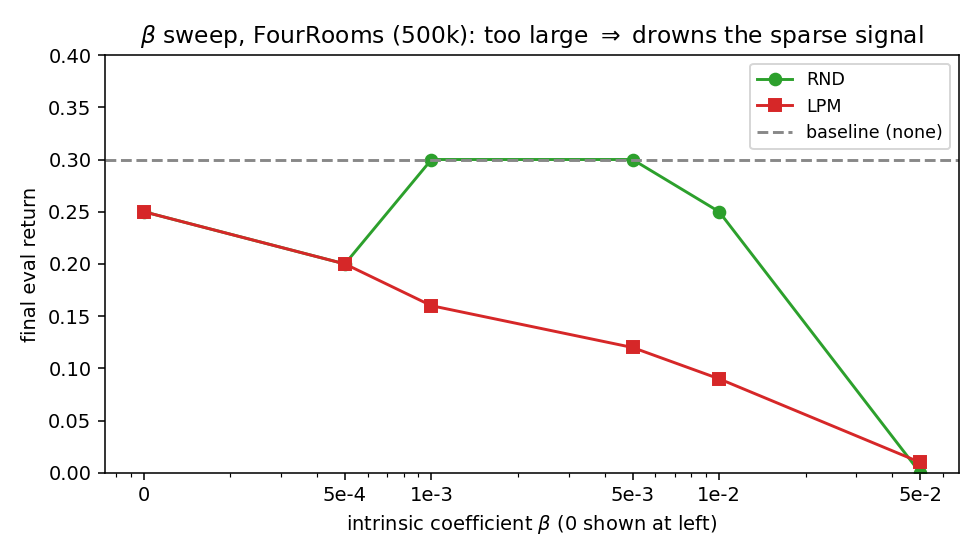
\includegraphics[width=0.72\textwidth]{fig2_beta_sweep.png}
\caption{$\beta$ sweep on FourRooms (500k). RND rises to a sweet spot ($\beta\!\approx\!0.001$--$0.005$,
matching the baseline) then collapses to $0$ at $\beta{=}0.05$; LPM declines monotonically.}
\label{fig:beta}\end{figure}

At $\beta{=}0.05$ the per-episode \emph{intrinsic} reward was $100$--$700\times$ the sparse extrinsic
reward, so the policy optimises novelty and never learns the goal (eval $\to 0$). The usable band is
$\sim$0.001--0.005. On the \emph{hard} env a slightly larger $\beta$ is needed to drive exploration,
but too large still prevents convergence to exploitation: RND on MultiRoom-N6 only converges at
$\beta{=}0.005$ (eval $0.28$); at $\beta{=}0.01$/$0.05$ it reaches the goal during training but never
settles into a reliable deterministic policy (eval $\approx 0$). \textbf{Takeaway:} $\beta$ is
environment-dependent --- small when intrinsic reward is a nuisance, larger when it is essential, with
a sweet spot in between. \note{Slide 3.3.}

\section{Does intrinsic reward beat the baseline? (RQ3)}
\begin{figure}[h]\centering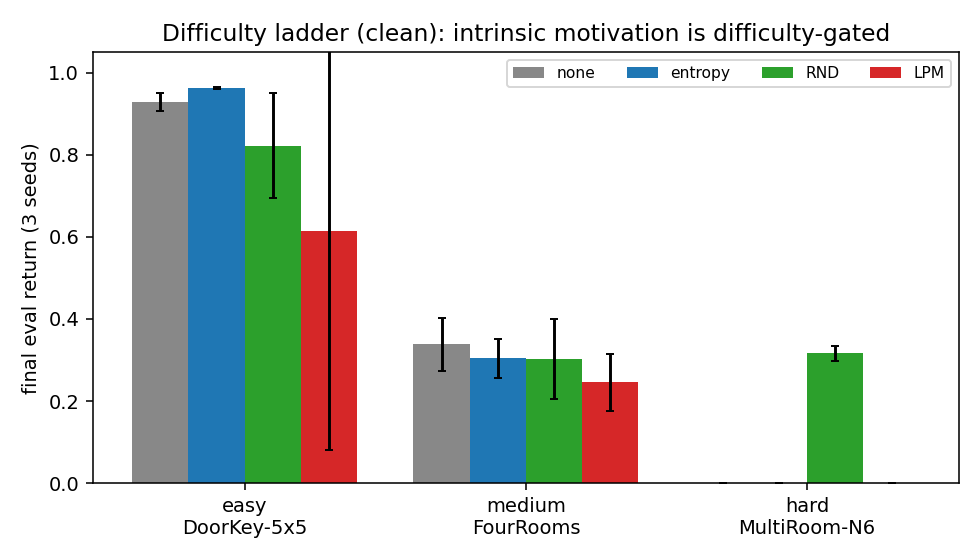
\includegraphics[width=0.78\textwidth]{fig1_difficulty_ladder.png}
\caption{Difficulty ladder, clean, final eval return. Easy/medium: the baseline already
solves/explores; intrinsic is unneeded (and slightly hurts). Hard MultiRoom-N6: only RND reaches the
goal.}\label{fig:ladder}\end{figure}

\begin{table}[h]\centering
\begin{tabular}{lcccc}
\toprule
env (clean) & \textsc{none} & \textsc{entropy} & \textsc{rnd} & \textsc{lpm} \\
\midrule
DoorKey-5x5 (easy)   & 0.93 & 0.96 & 0.82 & 0.61 \\
FourRooms (medium)   & 0.34 & 0.30 & 0.30 & 0.25 \\
MultiRoom-N6 (hard)  & 0.00 & 0.00 & \textbf{0.32} & 0.00 \\
\bottomrule
\end{tabular}
\caption{Final eval return (mean, 3 seeds). \textbf{Intrinsic motivation is difficulty-gated.}}
\label{tab:ladder}\end{table}

Intrinsic motivation's benefit appears \emph{only} when exploration is genuinely hard. On easy and
medium tasks the PPO baseline explores adequately on its own and any bonus slightly degrades it; on
hard MultiRoom-N6 the baseline and entropy never reach the goal, while \textbf{RND solves it reliably}
(0.32, all seeds). \note{Slide 3.4.}

\paragraph{Why RND $>$ LPM on clean hard exploration.} Per-episode intrinsic magnitudes show the
mechanism: RND's bonus is \emph{always positive} (mean $=$ abs), a consistent directional drive toward
novel states; LPM's bonus is \emph{signed} and nets $\approx 0$ per episode (mean $+0.08$ vs.\ abs
$0.33$), giving no coherent exploration push --- so the LPM agent behaves like the baseline and never
explores out. Raising $\beta$ scales LPM's oscillation amplitude, not its directionality, so no
$\beta$ rescues it. This is LPM's designed trade-off: its learning-progress signal goes to $0$ both
for unpredictable noise (its robustness virtue, next section) \emph{and} for already-learned local
dynamics (so it under-explores clean hard tasks).

\section{Noise robustness: LPM vs.\ RND (RQ4)}
\begin{figure}[h]\centering
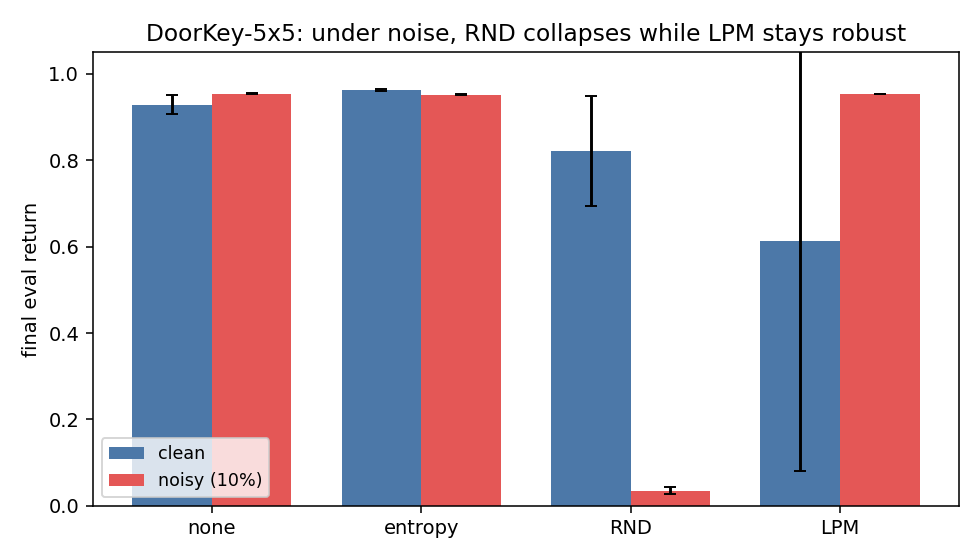
\includegraphics[width=0.49\textwidth]{fig3_doorkey_noise.png}\hfill
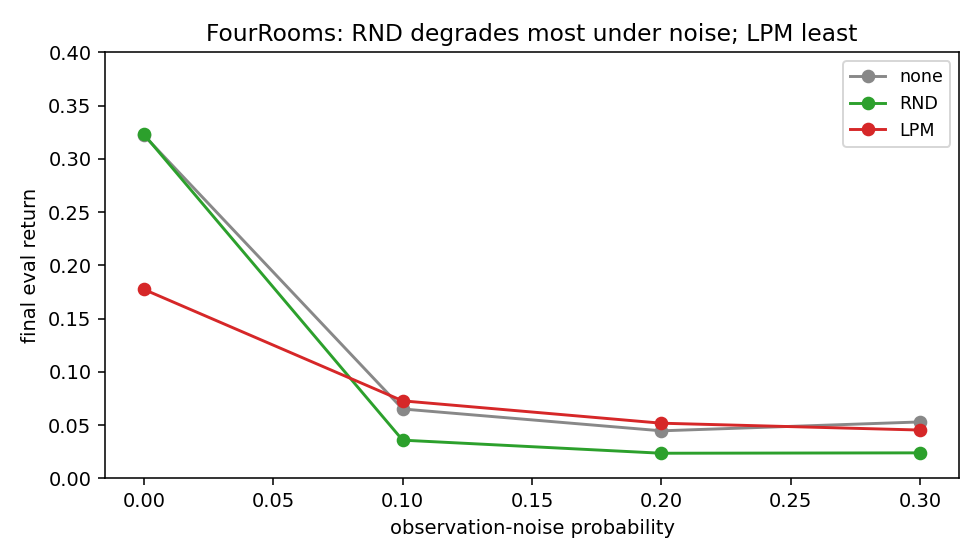
\includegraphics[width=0.49\textwidth]{fig4_fourrooms_noise.png}
\caption{\textbf{Left:} DoorKey-5x5 clean vs.\ 10\% observation noise --- RND collapses
($0.82\to0.035$), LPM stays robust ($0.61\to0.95$, like the baseline). \textbf{Right:} FourRooms
degradation vs.\ noise probability --- RND falls off the most, LPM the least.}\label{fig:noise}\end{figure}

\begin{table}[h]\centering
\begin{tabular}{lcc}
\toprule
DoorKey-5x5 & clean & noisy (10\%)\\
\midrule
\textsc{none} & 0.93 & 0.95\\
\textsc{entropy} & 0.96 & 0.95\\
\textsc{rnd} & 0.82 & \textbf{0.035}\\
\textsc{lpm} & 0.61 & \textbf{0.95}\\
\bottomrule
\end{tabular}
\caption{The cleanest noise-robustness result. DoorKey-5x5 is small enough that 10\% noise does not
stop \textsc{none}/\textsc{entropy}/\textsc{lpm} from solving --- which \emph{isolates} the
intrinsic-reward noise-vulnerability: only RND is destroyed.}\label{tab:doorkeynoise}\end{table}

Observation noise makes every state look ``novel,'' so RND's prediction-error bonus stays high and the
agent chases noise instead of the goal; LPM's learning-progress signal stays near $0$ on unlearnable
noise, so LPM is not distracted and effectively reverts to the (working) base policy. DoorKey-5x5
(Table~\ref{tab:doorkeynoise}) isolates this cleanly because the task is easy enough that noisy
perception alone does not break it. On FourRooms the same \emph{ordering} holds (RND hurt most, LPM
least, Fig.~\ref{fig:noise} right) but the global noise also degrades the policy's perception, so all
methods fall to $\approx 0.05$ --- ``LPM degrades less,'' not ``LPM stays solved.'' On hard
MultiRoom-N6, noise breaks perception for everyone (RND's clean $0.32 \to 0$). \note{Slides 3.4/3.6.}

\section{Agent traces (slide 3.5)}
Animated GIFs live in \texttt{expr\_data/minigrid/figures/traces/}; representative film-strips below.
\begin{figure}[h]\centering
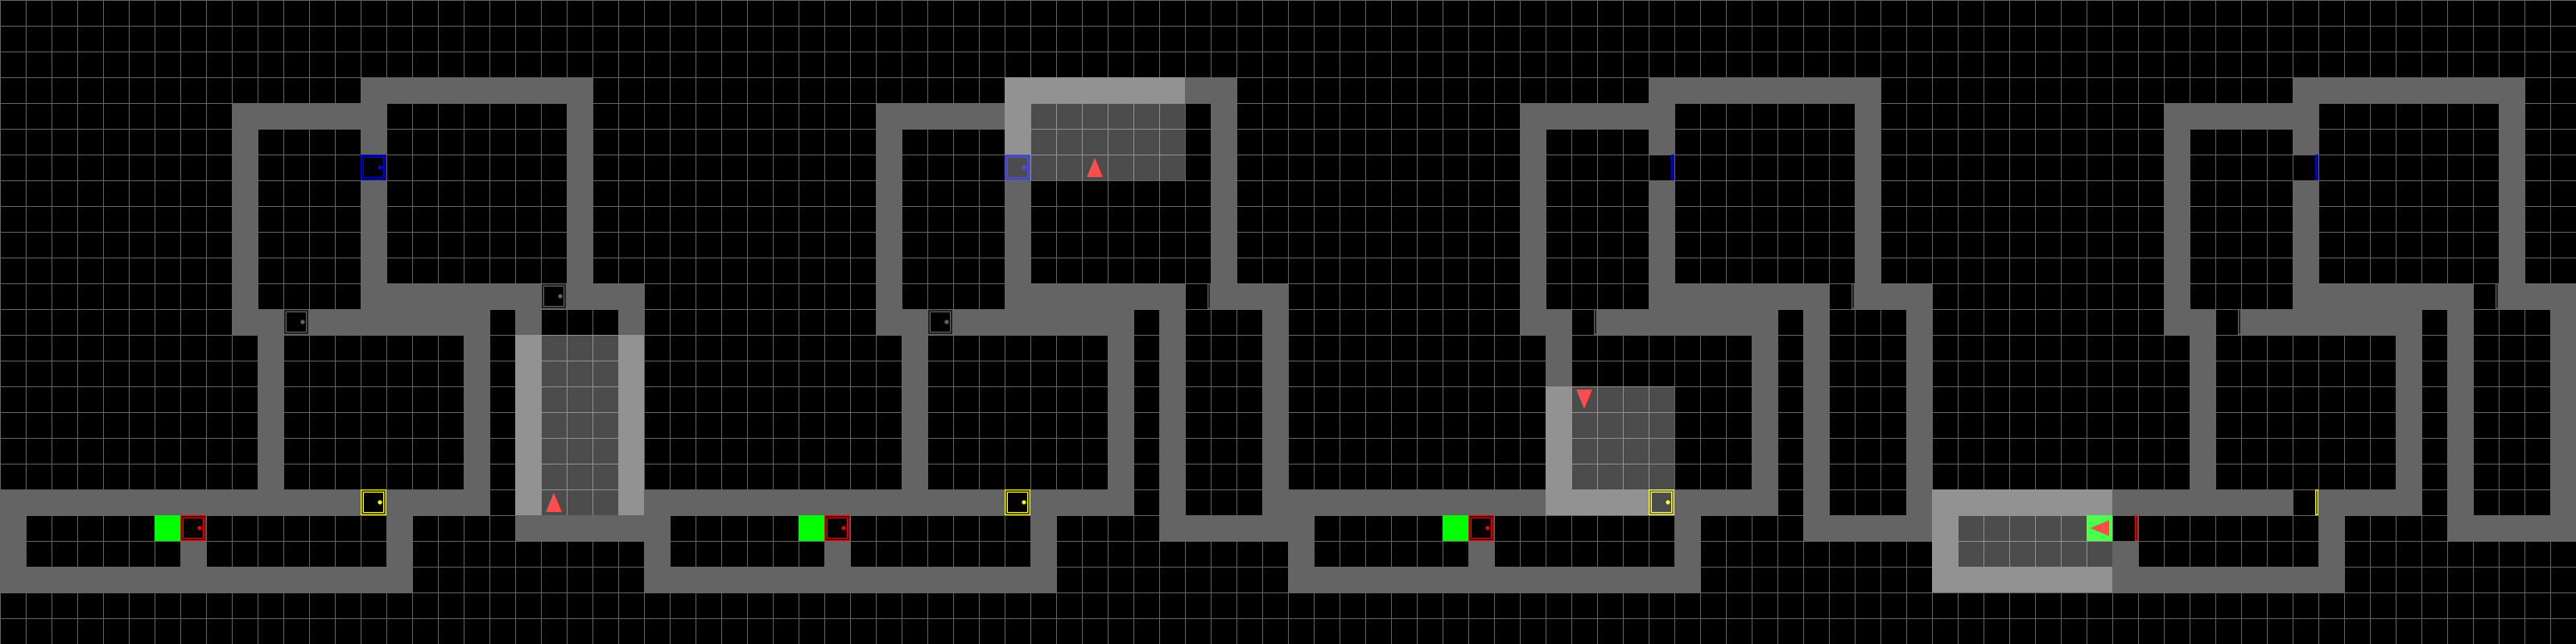
\includegraphics[width=0.9\textwidth]{strip_multiroom_rnd_solves.png}\\[2pt]
\note{Hard exploration --- RND threads through the MultiRoom-N6 chain to the goal (reward 0.54).}\\[6pt]
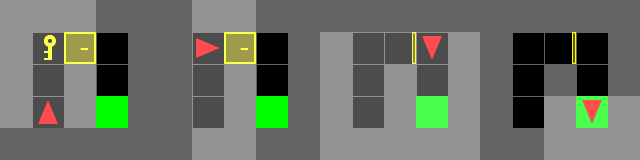
\includegraphics[width=0.49\textwidth]{strip_doorkey_lpm_noisy_solves.png}\hfill

\includegraphics[width=0.49\textwidth]{strip_doorkey_rnd_noisy_fails.png}\\[2pt]
\note{Noise robustness on DoorKey-5x5 (10\% noise): LPM (left) solves in $\sim$13 steps; RND (right)
wanders the full budget and fails.}
\caption{Trajectory film-strips (evenly-spaced frames). Top: intrinsic motivation enables hard
exploration. Bottom: LPM is noise-robust where RND is not.}\label{fig:traces}\end{figure}

\section{Conclusions --- answers to the research questions}
\begin{enumerate}[leftmargin=2em]
\item[\textbf{RQ1}] \emph{What do the LPM-paper experiments say about exploration metrics?}
Coverage (MiniWorld) is a poor metric in extrinsic-free settings (a uniform-random policy maximises
it). In MiniGrid we use \emph{task success / return}, which actually discriminates exploration quality.
\item[\textbf{RQ2}] \emph{Correct way to mix extrinsic/intrinsic; $\beta$ too small/large?}
$\beta$ too large drowns the sparse reward ($\to 0$); too small is ignored. Usable $\sim$0.001--0.005,
environment-dependent; on hard tasks there is a sweet spot ($\approx0.005$ for RND) between
under-exploring and never-converging (Fig.~\ref{fig:beta}).
\item[\textbf{RQ3}] \emph{Does intrinsic reward beat baselines on sparse MiniGrid?}
Only when exploration is hard: \textbf{yes, decisively, on MultiRoom-N6 (RND $0.32$ vs.\ $0.0$)}; no on
easy/medium where the baseline suffices (Fig.~\ref{fig:ladder}). RND $>$ LPM on clean hard exploration.
\item[\textbf{RQ4}] \emph{Does LPM generalise to other noise (beyond the MiniWorld noisy-TV)?}
Yes --- \textbf{LPM is noise-robust and RND noise-vulnerable}, cleanest on DoorKey-5x5
(RND $0.82\!\to\!0.035$, LPM $\to\!0.95$; Table~\ref{tab:doorkeynoise}). This reproduces the paper's
claim in a second, symbolic-observation domain.
\end{enumerate}

\noindent\textbf{One-line story for the deck:} \emph{intrinsic motivation buys you hard-exploration
ability (RND) at the price of noise-fragility; LPM trades exploration aggressiveness for
noise-robustness} --- and $\beta$ must be tuned or it drowns the task.

\section*{Slide-deck mapping (SPEC \S3 ``Intrinsic Reward and LPM'')}
\begin{itemize}[leftmargin=2em,itemsep=1pt]
\item 3.1 Environments / 3.2 Model \& setup $\to$ \S1.
\item 3.3 $\beta$ sweep $\to$ \S2, Fig.~\ref{fig:beta}.
\item 3.4 Success rate across envs (clean and noisy) $\to$ \S3--\S4, Fig.~\ref{fig:ladder},
Table~\ref{tab:ladder}, Fig.~\ref{fig:noise}.
\item 3.5 Trace demonstrations $\to$ \S5, Fig.~\ref{fig:traces}.
\item 3.6 LPM vs.\ RND, clean and noisy performance gap $\to$ \S3 (clean: RND$>$LPM) + \S4
(noisy: LPM$>$RND) --- the rank flip is the punchline.
\end{itemize}

\appendix
\section{Reproducibility \& data}
Code: \texttt{minigrid\_exp/} (vendored + extended from Youssef's
\texttt{minigrid\_intrinsic\_reward}). Raw data, tables, figures and trace GIFs:
\texttt{expr\_data/minigrid/} with a running log in \texttt{FINDINGS.md}.
\textbf{Compute note:} the 128-core box SIGKILLs any single process after $\sim$18~min, so long runs
use chunked checkpoint--resume training (\texttt{train\_one --chunk-steps}, resume via
\texttt{PPO.load}) driven by a meta-loop re-invoking \texttt{run\_grid.py} (\texttt{ThreadPoolExecutor});
each chunk finishes under the limit and the idle driver survives. Grids:
\texttt{run\_grid.py --envs ... --methods rnd lpm --betas ... --noise-probs ... --seeds 1 2 3}.
\textbf{Caveats:} (a) the MiniGrid noise is \emph{global} per-element corruption, not a localised
noisy-TV distractor; a localised variant would be a cleaner analogue. (b) LPM under-explores clean
hard tasks here, so the clean LPM-vs-RND gap is RND-favourable; the noise result is the LPM-favourable
half. (c) 3 seeds --- DoorKey-clean LPM is bimodal (high variance).
\end{document}
